\documentclass[12pt]{article}
\usepackage{apacite}
\usepackage{hyperref}
\usepackage{natbib}
\usepackage{amsmath, amssymb}
\usepackage{titling}
\usepackage{layout}
\usepackage{fontspec}
\usepackage[nottoc]{tocbibind}
\settocbibname{References}
\setlength\topmargin{0pt}
\addtolength\topmargin{-\headheight}
\addtolength\topmargin{-\headsep}
\setlength\oddsidemargin{0pt}
\setlength\textwidth{\paperwidth}
\addtolength\textwidth{-2in}
\setlength\textheight{\paperheight}
\addtolength\textheight{-2in}
\usepackage{layout}
\usepackage{titling}
\linespread{1.25}
\usepackage{pgfplots}
\pgfplotsset{compat = newest}
\usetikzlibrary{positioning, arrows.meta}
\usepgfplotslibrary{fillbetween}
\usepackage{color,pxfonts,fix-cm}
\usepackage[mathletters]{ucs}
\usepackage[T1]{fontenc}
\usepackage{pict2e}
\usepackage{wasysym}
\usepackage[english]{babel}
\usepackage{tikz}
\numberwithin{equation}{subsection}
\let\oldsection\section% Store \section
\renewcommand{\section}{% Update \section
  \renewcommand{\theequation}{\thesection.\arabic{equation}}% Update equation number
  \oldsection}% Regular \section
\let\oldsubsection\subsection% Store \subsection
\renewcommand{\subsection}{% Update \subsection
  \renewcommand{\theequation}{\thesubsection.\arabic{equation}}% Update equation number
  \oldsubsection}% Regular \subsection

\newcommand{\subtitle}[1]{%
  \posttitle{%
    \par\end{center}
    \begin{center}\large#1\end{center}
    \vskip0.5em}%
}
\usepackage{multirow,booktabs,setspace,caption}
\usepackage{tikz}
\renewcommand{\contentsname}{Table of Contents}

\DeclareCaptionLabelSeparator*{spaced}{\\[2ex]}
\captionsetup[table]{textfont=it,format=plain,justification=justified,
  singlelinecheck=false,labelsep=spaced,skip=0pt}
\captionsetup[figure]{labelsep=period,labelfont = bf,justification=justified,
  singlelinecheck=false,font=doublespacing}
 

\setmainfont{Times New Roman}
\begin{document}


\newpage
\renewcommand{\BRetrievedFrom}{}
\pagenumbering{Roman}
\begin{abstract} \noindent This paper analyzes in-depth Antoine Augustin Cournot's contribution to economic theory. It is mainly developed on two levels, the first one descriptive which intends to approach the theories stipulated by Cournot in his book of 1838, \nocite{cournot1838recherches}\emph{Recherches sur les principes mathématiques de la théorie des richesses}, in the most faithful and truthful way possible. The second level leads instead to the discovery of deep connections between current economic theory and Cournot's theories, revealing through algebraic calculus how despite the different formulation the current economic equations for monopoly and duopoly obtain the same results as Cournot's theories. Analyzing subsequently the duopoly theory of Stackelberg, who was inspired by Cournot's duopoly, we get interesting results regarding the application of the two theories in the case where the two companies have identical constant marginal costs with a linear inverse demand. Namely that the duopoly of Cournot is more efficient in maximizing the total profits of the market and minimizing the consumer surplus.
\end{abstract}
\newpage
\tableofcontents
\newpage
\clearpage
\pagenumbering{arabic}
\section{Introduction}
\label{sec:intro}
Economics as a science ``is not defined by an object of study. Instead, it defines itself by a particular perspective from which it tries to make sense of the social world: scarcity" \cite[p. 4]{Kolmar_2022}. Scarcity has incentivized so many humans to theorize the most unpredictable ways while trying to explain the functioning of the world. Scarcity is also the starting point for one of the most important economists who ever lived, namely Antoine Augustin Cournot. Born in Gray, France, on August 28, 1801 \cite[p. V]{cournot1897researches} he is best known for his duopoly model, which is still taught in economics departments around the world. During his life the most important event was certainly the publication in 1838 of \emph{Recherches sur les principes mathématiques de la théorie des richesses}, which translated into English means Researches into the mathematical principles of the theory of wealth, and that is the book on which we base a large part of this research, being able to outline what has been his contribution to economic theory. Cournot died on March 31, 1878, in Paris, one year after his last publication, named \nocite{cournot1877recherches}\emph{Revue sommaire des doctrines économiques}, he was an academic all his life, first as a student, then as a professor, subsequently as a rector, and finally as a pensioner, publishing during all these years economical and philosophical books \cite[p. V]{cournot1897researches}.

Cournot in his time had understood that ``the public is so tired of theories and systems that now the demand is for so-called \emph{positive} matter" \cite[p.1]{cournot1897researches}, i.e. empirical evidence, real data and theories that can explain through mathematics why reality is the way it is. Precisely for this reason he begins to stipulate various economic theories, some more influential and others less so, searching for economic dogmas that can be true and above all empirically real, in order to provide the mathematical tools to economic science to explain market dynamics. Scarcity in fact, refers in its economic meaning, to those ``situations where the wants exceed the means" \cite[p.4]{Kolmar_2022}, and in Cournot's era the public wanted answers, but did not yet have the means to obtain them. Cournot provides the means to get them, and it is surprisingly brilliant the way he loosely stipulates his various theories. This paper aims to take an in-depth look at the reasoning that brought them to light, and more importantly, how his theories have contributed to economic theory.

The first part is dedicated exclusively to Cournot's theories. The second part instead fully reflects the central question of the paper, comparing today's theories and Cournot's, specifically deepening how the latter reflects on the former and how much theories that are more than 150 years old  are still valid in the present. In addition, the second part also digresses on von Stackelberg's duopoly model, which takes its cue from Cournot's duopoly model, analyzing possibles advantages and disadvantages of both duopoly forms.
\newpage
\section{Economic Theory -- Determination of Prices}
\label{sec:eco}
Cournout was not only a philosopher or an economic scientist, he was and is a character who will always be fundamental for everything related to current and future economic theory. Owing to him economics has finally been able to find a purely mathematical meaning that can both describe the current reality, thus the present, the past at an empirical level, and the future, meaning the economic projections that are possible through his models. In his first work \emph{Recherches sur les principes mathématiques de la théorie des richesses} (\citeyear{cournot1838recherches}), Cournot finally manages to give a mathematical imprint to all those hypothesis that had been only theorized up to that moment and therefore had a purely descriptive character without any way to be implemented at a real level.

In the following subsections \ref{sec:demand}, \ref{sec:mono}, \ref{sec:oligo}, the paper analyzes his main innovations in economic theory, taking cue from the first translation available to us in english \citep{cournot1897researches} of Cournot's aforementioned book. The whole section \ref{sec:eco} focuses essentially on three chapters of his book which is instead composed of twelve chapters. The aim of this section as is stated in the title is to take a look more deeply of the various formulas that led Cournot to the determination of prices in various market forms. Cournot's mathematical intuitions about the determination of prices are still considered pillars of economic science, having not been appreciated in a sufficiently important way during his time at the beginning of the nineteenth century, but rediscovered and reformulated in the manner that the formulas are known as of today by Marshall (\citeyear{marshall_principles_1988}) at the end of the nineteenth century.
\subsection{Demand and Supply}
\label{sec:demand}
One reason that made Cournot one of the greatest economic scientists of all time is what is discussed in this chapter, namely his ``theory of exchangeable values'' \cite[p. 44]{cournot1897researches}. To accomplish it Cournot relied on the utilitarian theory which stipulated that every human seeks to derive the maximum benefit, or maximum utility, from their goods or labor. On this point, however, Cournot hesitates, expressing disappointment for what has been done by other economists, stating that this proposition was ``presented to us, we will not say falsely, but in a manner which is really meaningless'' \cite[p. 44]{cournot1897researches}. In his fourth chapter entitled ``Of the Law of Demand'' \cite[p. 44]{cournot1897researches} Cournot tries to understand what is this quantity demanded, and how it can vary with changes in price. He then states that the demand is nothing more than a synonym of sales \cite[p. 46]{cournot1897researches}, thus not taking in his theory in any way account of ``any demand which does not result in a sale'' \cite[p. 46]{cournot1897researches}. Thanks to this axiom he deduces that the demand increases as the price decreases, or that the demand is inversely proportional to price \cite[p.46]{cournot1897researches}. Various other statements are made by Cournot that theorize what today we commonly call elasticity of demand, comparing for example manufactured products, whose demand changes more rapidly than the slowness, and therefore inelasticity, with which demand can vary with respect to products of first necessity, but surprisingly states, even with respect to less necessary and more futile products \cite[p. 46]{cournot1897researches}.

But now in this subsection comes the most interesting part, which really concerns this research with respect to Cournot's contribution not only theoretical, but to his mathematical insights that revolutionized economic science. Cournot et al. (\citeyear[p. 47]{cournot1897researches}) in fact states that this demand, which he calls $D$, is for each good or article, a function $F(p)$ of the price $p$ of this said article. Posing the question of what form this function has, he states rhetorically that it would mean knowing the law of demand. He assumes in fact that $F(p)$, that nowadays is called the demand function, is a continuous function, supporting this argument with the idea that obviously it would not be continuous if a limited number of consumers were involved, but surely it becomes continuous as the portion of the market analyzed will include more and more individuals, and therefore more and more ``combinations of needs, of fortunes, or even of caprices, [\ldots] among consumers'' \cite[p. 50]{cournot1897researches}.

Here we report one of his first fundamental intuitions about all the mathematical economy that is postulated in his book, which is directly related to the assumption of continuity of the demand function: ``\emph{the variations of the demand will be sensibly proportional to the variations in price so long as these last are small fractions of the original price}'' \cite[p. 50]{cournot1897researches}. Assuming that the period in which the market is analyzed is annual, Cournot states that $p$ must ``denote annual average price'' \cite[p. 52]{cournot1897researches}, and that the curve of the function $F$ must be the ``average of all the curves which would represent this function at different times of the year'' \cite[p. 52]{cournot1897researches}. The other function that Cournot moulds is $pF(p)$, ``which expresses the total value of the quantity annually sold, must be continuous also'' \cite[p. 52]{cournot1897researches} because of the continuity of the above mentioned $F(p)$.

Given the inverse proportionality of $F(p)$ with respect to price, the function $pF(p)$ ``at first increases, and then decreases as $p$ increases'' \cite[p. 53]{cournot1897researches}, therefore according to the Weierstrass theorem there is a value of $p$ according to which the function $pF(p)$ has a maximum. This maximum according to Cournot et al. (\citeyear[p. 53]{cournot1897researches}) is described by the equation \begin{equation}
\label{eq:Max_C}
F(p) + pF'(p) = 0.
\end{equation}

The value of $p$ which will solve equation (\ref{eq:Max_C}) is fundamental for Cournot for another reason as well, that is to be able to determine if the current price of an analyzed good is greater or lesser than the price which would optimize the value of the annual quantity \cite[p. 53]{cournot1897researches}. Cournot therefore supposes that the price becomes $p + \Delta p$ and therefore according to the above described law of demand, the demand becomes $D - \Delta D$. If therefore the increase of $\Delta p$ in the price increases the total product $pF(p)$ then, the two values $p$ and $p + \Delta p$ will therefore be below the optimal price that maximizes $pF(p)$, on the contrary if $\Delta p$ decreases the total product $pF(p)$, then the price will be higher than the optimal one \citep[p. 53-54]{cournot1897researches}. Through this intuition he suggests that trade statistics should be made in such a way as to divide two main categories of products, those whose price is lower than the optimal one and vice versa. Because ``many economic problems have different solutions, according as the article in question belongs to one or the other of these two categories'' \cite[p. 54]{cournot1897researches}. Cournot is not sufficiently naive as not to consider the possibility of the existence of multiple maxima or minima belonging to the function $pF(p)$, but excludes \emph{a priori} that their existence can really be reflected empirically, thus considering all pricing problems as equal with respect to the uniqueness of the existence of a single maximum of the function $pF(p)$ \citep[p. 55]{cournot1897researches}. 

In the following subsection we try to describe what are the mathematics theorized by Cournot for the determination of prices, taking what for him is ``the simplest hypothesis for the purpose of investigating by what laws prices are fixed'' \cite[p. 55]{cournot1897researches}, namely the monopoly.
\subsection{Monopoly Without Price Discrimination}
\label{sec:mono}
Cournot means the monopoly as it is understood today, so that ``the production of an article is one man's hands'' \cite[p. 55]{cournot1897researches}. As it has been explained in subsection \ref{sec:demand}, that equation (\ref{eq:Max_C}) determines the maximum possible value for $pF(p)$ with respect to a value of $p$, thus the objective for the monopolists is to achieve the value of $p$ that maximizes $pF(p)$. Obviously Cournot knows that there must also be a demand $D$ that precisely equals the quantity of goods produced to make the equation (\ref{eq:Max_C}) applicable. Taking the same example used by Cournot, a source of water, and denoting with $\Delta$ the quantity of liters produced annually, equation (\ref{eq:Max_C}) can be reduced to $F(p) = \Delta p$, obtaining the ``price per liter which must finally be fixed by the competitor'' \cite[p. 57]{cournot1897researches}.

In the first case, however, there is no production cost, which in fact Cournot ignores for didactic and reasoning reasons, while now instead the second case that is described also contains production or labor costs that cannot be ignored. In this way the profit of the monopolist will no longer be $pF(p)$, which is the gross profit, instead it will be equal to the net profit, or the value of $pF(p)$ reduced by the annual costs necessary to produce the quantity demanded, or $\phi (D)$. Because of these production costs burdening the monopolist Cournot stipulates another equation for pricing, with the possibily to substitute $\frac{dD}{dp}$ with $\frac{1}{f'(D)}$ if wanted, which is \citep[p. 57]{cournot1897researches} \begin{equation}
\label{eq:Max_M}
D + \frac{dD}{dp} \cdot \left[p-\frac{d[\phi (D)}{dD}\right] = 0.
\end{equation}

Another case that Cournot analyzes concerning monopoly is that of the ``limitation of the productive forces'' \cite[p. 58]{cournot1897researches}, which according to him should therefore limit the ability of the monopolist to take maximum advantage from equation (\ref{eq:Max_M}), thus not allowing to reach the maximum net profit. In this case $\Delta$ is no longer be the number of liters of water produced but rather the maximum amount of production possible derived from the limitation of productive forces, consequently the equation $F(p) = \Delta$ determines the price, not taking however into account possible production costs. 

Returning to the case in which the existence of a price $p$ that succeeds in maximizing the monopolist's profit is granted, Cournot  formulates one of the maximum triads of current economic theory, applicable both to perfect competition and to monopoly and oligopoly, i.e. that $\frac{d[\phi(D)]}{dD}$, nowadays called marginal costs, must necessarily be positive, because ``it would be absurd that the \emph{absolute} expense of production should decrease as production increases'' \cite[p. 59]{cournot1897researches}. This condition is applied in all types of microeconomics problems and cannot be false, else most, if not all, of the present theories would turn out to be not applicable. In addition it is also stated that $p > \frac{d[\phi(D)]}{dD}$, which by reflecting on the relationships established between the increase in expenses and that of profits claims a limit at the same time basic and innovative, namely that the monopolist will stop increasing its production ``when the increase in expense exceeds the increase in receipts'' \cite[p. 59]{cournot1897researches}. 

Cournot concedes much about the analysis of the behavior of $\phi '(D)$ with respect to the type of product involved, e.g. he states, as economic theory nowadays claims, that for manufactured products $\phi '(D)$, i.e., the marginal costs, decrease as the quantity produced increases. The inverse is true for real estate, i.e. the function ``$\phi '(D)$  increases with $D$'' \cite[p. 60]{cournot1897researches}. However, there is another fundamental case that Cournot analyzes in depth, and that is the case in which $\phi (D)$ is constant, and consequently $\phi '(D) = 0$, thus modifying equation (\ref{eq:Max_M}) and making it become $D+\frac{dD}{dp}*(p-g) = 0$. If till now price has been always determined with regard to $\phi '(D)$ having a variable or fixed value, from now on $p$ must reflect the behavior of $\phi '(D)$  as a null value. In this case the constant $g$ in the above equation disappears, therefore equation (\ref{eq:Max_M}) will become equal to equation (\ref{eq:Max_C}), as if there were no costs \citep[p. 59-61]{cournot1897researches}.

As it can already be deduced from the last paragraph, it seems obvious that due to the behavior of equation (\ref{eq:Max_M}), as production costs increase, the price set by the monopolist will increase. Cournot, however, because of his obsession for being able to explain economic science through mathematics, wants to show that this is not only an obvious behavior, but it is unavoidable and indisputable, therefore claimed from a mathematical demonstration. If $p_0$ is the solution of equation (\ref{eq:Max_M}), changing $\phi '(D)=\phi '[F(p)]$, from the relation of subsection \ref{sec:demand} $D = F(p)$, with $\psi(p)$ equation (\ref{eq:Max_M}) becomes \citep[p. 61]{cournot1897researches} \begin{equation}
F(p) + F'(p)\left[p - \phi(p)\right] = 0,
\end{equation} and if the quantity demanded and the price vary correspondingly by $u$ and $\delta$, becoming $\psi (p) + u$ and $p_0 + \delta$, the following relationship can be established between $u$ and $\delta$ \citep[p. 62]{cournot1897researches}: \begin{equation}
\left \{ F'(p_0)[2 - \psi '(p_0)] + F''(p_0)[p_0 - \psi (p_0)]\right \} \delta - uF'(p_0) = 0.
\end{equation} Cournot, however, states that ``$\delta$ is necessarily negative'' \cite[p. 62]{cournot1897researches} because if it were positive, $p_0$ would no longer correspond with the maximum of the function $pF(p)-\phi (D)$ but with the minimum. In general, therefore, the change in price is in the same direction, whether positive or negative, of the change in production costs, or ``the increment of $\delta$ is of the same sign as the increase in $u$'' \cite[p. 62]{cournot1897researches}.
\subsection{Oligopoly}
\label{sec:oligo}
Cournot initially did not call oligopoly the form of the market that today is known as such, but ``competition of producers'' \cite[p. 79]{cournot1897researches}. Based on the aforementioned example of the spring he constructs a situation were two producers supply the same market, with $D_1$ and $D_2$ reflecting the sales of the respective springs, and $D_1+D_2 = D$ the total sales, defined by the equation $D = F(p)$. Consequently, the revenues made by the oligopolists will be $pD_1$ and $pD_2$, both maximized by each of them independently, as when they would reach an agreement, the market structure would take the form of a monopoly \cite[p. 79-80]{cournot1897researches}. Cournot now has the first intuition that will lead to the concept of the determination of prices that we know today, in fact, he states that ``instead of adopting $D = F(p)$ as before, in this case [of oligopoly] it will be convenient to adopt the inverse notation $p=f(D)$'' \cite[p. 80]{cournot1897researches}. Cournot et al. (\citeyear[p. 79-80]{cournot1897researches}) defines the inverse demand notation of what today is known as $p=P(y)$, consequently also redefining the profits of the two oligopolists with inverse demand function $p=f(D)$, making them become $D_1 \cdot f(D_1+D_2)$ and $D_2 \cdot f(D_1+D_2)$. The profit functions of the two oligopolists do not have one, instead two variables, since $D$ is defined by the above equation $D_1+D_2 = D$, which is a fundamental step in determining the optimal price.

As far as the price determination is concerned, each of the two producers will not have direct influence on the adversary, therefore the only way left to go is to determine its optimal quantity $D_2$ after the quantity of the competitor $D_1$ has been decided. Consequently then the same will happen for $D_1$ which will be recalibrated to be optimal and so on. At the mathematical level Cournot therefore assumes that $D_1$ will be determined with respect to $D_2$ by the equation \citep[p. 80]{cournot1897researches} \begin{equation*}
\frac{d \left[D_1f(D_1 + D_2)\right]}{dD_1} = 0,
\end{equation*} which will resemble the determination of $D_2$ with respect to $D_1$, i.e. \begin{equation*}
\frac{d \left[D_2f(D_1 + D_2)\right]}{dD_2} = 0.
\end{equation*} Consequently Cournot discovers the first equations, again with respect to the situation in which there are no production costs, which determine $D_1$, $D_2$ and $p$, namely \citep[p. 81]{cournot1897researches} \begin{equation}
\label{eq:duo1}
f(D_1 + D_2) + D_1f'(D_1 + D_2) = 0,
\end{equation} \begin{equation}
\label{eq:duo2}
f(D_1 + D_2) + D_2f'(D_1 + D_2) = 0.
\end{equation} From equation (\ref{eq:duo1}) and (\ref{eq:duo2}) Cournot derives the first values for $D_1$ and $D_2$ posing the equality $D_1 = D_2$, which is technically correct considering the similarity that the oligopolistic market requires between the producers goods to be considered as such, obtaining the equation $2f(D)+Df'(D)=0$ \citep[p. 82]{cournot1897researches}, which recalibrated becomes $D + 2p \cdot \frac{dD}{dp} = 0$. On the other hand, if the two sources would have belonged to the same monopolist, or if the oligopolists had come at an agreement, the equation for determining the price $p$ would have become $D + p \cdot \frac{dD}{dp} = 0$, and clearly the latter equation would have brought the price and quantity to the optimum maximizing the profit $Dp$. The main reason why this agreement does not happen is because the producer that fixes the quantity at a later stage can take advantage of it with a short-term advantage. Obviously this behavior will twist against the one that abused it, due to the subsequent reaction of the manufacturer who set the quantity in advance. As a consequence these ``reactions, far from bringing both producers nearer to the original condition [of monopoly]'' \cite[p. 83]{cournot1897researches} will consequently bring instability to the equilibrium, and precisely because of this, the equilibrium of the oligopoly is never firm.

So far it has only been described the condition of duopoly, a case of oligopoly that it is useful to explain before being able to subsequently introduce the oligopoly with $n$ producers, because starting from the same mathematical logic can be easily deduced as it can also be applied to the oligopoly with $n$ producers. If in fact in the situation of duopoly the equilibrium condition was \citep[p. 82]{cournot1897researches} \begin{equation*}
D + 2p \cdot \frac{dD}{dp} = 0,
\end{equation*} in the condition of oligopoly with $n$ producers it becomes \citep[p. 84]{cournot1897researches} \begin{equation*}
D + np \cdot \frac{dD}{dp} = 0.
\end{equation*} Cournot describing this formula describes an interesting property, that is that as $n$ increases, $p$ will be smaller and smaller \cite[p. 84]{cournot1897researches}. With the same reasoning as in the duopoly, it becomes a system composed by the $n$ equations \begin{equation}
\label{eq:np}
f(D) + D_if'(D) = 0,\quad i = 1,2, \ldots, n,
\end{equation} which added together will then give \citep[p. 85]{cournot1897researches} \begin{equation*}
nf(D) + nD_1f'(D) = 0.
\end{equation*} If instead the producers have to take into account the production costs $\phi_i(D_i)$ for $i = 1, 2, \ldots,n$ the system of equations (\ref{eq:np}) becomes \citep[p. 85]{cournot1897researches}\begin{equation}
\label{eq:2.7}
f(D) + D_if'(D) - \phi_i '(D) = 0,\quad i = 1,2, \ldots, n.
\end{equation}
Subtracting equation $i = 2$ with equation $i = 1$ we obtain \citep[p. 85]{cournot1897researches} \begin{equation}
\label{eq:duo_c}
D_1 - D_2 = \frac{1}{f'(D)} \cdot \left[\phi_1 '(D_1) - \phi_2 '(D_2) \right],
\end{equation} in addition due to the negativity of $\frac{1}{f'(D)}$, the inequality ratios between $D_1$ and $D_2$ and the corresponding marginal costs $\phi_1 'D_1$ and $\phi_2 'D_2$ are \citep[p. 85]{cournot1897researches}\begin{equation*}
D_1 \gtrless D_2 \text{ and } \phi_1 'D_1 \lessgtr \phi_2 'D_2,
\end{equation*} therefore, the quantity $D_1$ will be greater than $D_2$ whenever the marginal costs of production $\phi_1 '(D_1)$ will be less than $\phi_2 '(D_2)$. 

Adding up instead all the equations of the system \ref{eq:np} gives \citep[p. 86]{cournot1897researches} \begin{equation}
\label{eq:sum}
D + \frac{dD}{dp} \cdot \left[np - \sum\limits_{i=1}^n \phi_i '(D_i) \right] = 0.
\end{equation} Cournot compares equation (\ref{eq:sum}) with equation (\ref{eq:Max_M}), mathematically deducing that \citep[p. 87]{cournot1897researches}\begin{equation}
\label{eq:mc}
\frac{\sum\limits_{i=1}^n \phi_i '(D_i)}{n} > \phi '(D),
\end{equation} thus, precisely because of (\ref{eq:mc}) ``for a given value of $p$, or for the same production, the costs will always be greater for competing producers than they would be under a monopoly'' \cite[p. 87]{cournot1897researches}.
\newpage
\section{Influencing Economic Theory}
\label{sec:infl}
In this section we compare Cournot's theories and current theories, finding what are his main relevant findings that still exist in current economic theories, and what instead has been replaced because it was not deemed correct. 

In subsection \ref{sec:alg}, by hyping the theories described in Kolmar's book (\citeyear{Kolmar_2022}), we are able to gain a deeper understanding of the connections between current theory and Cournot's theory using algebraic calculus. 

Instead in subsection \ref{sec:stack}, we compare two different duopoly models, the Stackelberg's (\citeyear{von_Stackelberg_2011}) model and the Cournot's et. al. (\citeyear{cournot1897researches}) model, analyzing the market situation where the inverse demand is linear and the marginal costs are constant.
\subsection{Comparing Cournot's and Current Theories}
\label{sec:alg}
We first address what is for Cournot the simplest form of market, that is monopoly \cite[p. 55]{cournot1897researches}. We compare it with the current theory and see the similarities or discrepancies between the two theories. The first problem when one wants to compare two theories so far apart in time is the notation with which they are described, so initially we have to define all variables that we are going to use in a unique way. What Cournot defines with $D = F(p)$, that is the quantity, we call instead $y = y(p)$. The production costs, defined as $\phi (D)$, will instead be $C(y)$ and the sign of the derivative $d$ or simply $'$ is replaced by $\partial$ when using partial derivatives. Additionally the profit is denoted as $\pi$ and the consumer surplus, calculated only in section \ref{sec:duopoly_c_k}, is defined as $CS$.

The second problem that arises when comparing the two theories is one of reasoning, namely that Kolmar (\citeyear{Kolmar_2022}) uses throughout his mathematical theory the notation $P(y)$ and not $y(p)$, providing the various formulas with the inverse demand. To remedy this problem $P(y)$ is defined by \begin{equation}
\label{eq:inv_s}
P(y^z) = a - by^z, \quad z = C, K,
\end{equation}
and the demand is instead defined by \begin{equation}
\label{eq:supply}
y(p^z) = \frac{a - p^z}{b}, \quad z = C, K,
\end{equation}
such that the different formulas will match algebraically throughout this subsection and that with $C$ and $K$ we can compare the results obtained from the formulas of Cournot et al. (\citeyear{cournot1897researches}), denoted with $C$, and the ones obtained from Kolmar (\citeyear{Kolmar_2022}), denoted with $K$.

\subsubsection{Monopoly -- Algebraic Calculus}
\label{sec:m}
For the purpose of demonstration regarding monopoly marginal costs are  defined as \begin{equation}
\label{eq:costs_m}
C(y^z) = cy^z, \quad z = C, K.
\end{equation}
For Cournot et al. (\citeyear{cournot1897researches}) the equation that maximizes the profit of the monopolist is equation (\ref{eq:Max_M}) which transformed with the new notation becomes \begin{equation}
\label{eq:max_m_new}
y(p^C) + \frac{1}{P'(y^C)} \cdot \left[p - C'(y^C) \right] = 0, 
\end{equation}
for Kolmar (\citeyear[p. 406]{Kolmar_2022}) is instead \begin{equation}
\label{eq:max_m_kolmar}
P'(y^K) \cdot y^K + P(y^K) \cdot 1 - C'(y^K) = 0.
\end{equation}
Inserting (\ref{eq:inv_s}), (\ref{eq:supply}) and (\ref{eq:costs_m}) in (\ref{eq:max_m_new}) yields \begin{align*}
\frac{a - p^C}{b} + \left(\frac{1}{- b}\right) \cdot [p^C - cy^C] & = 0 \\
a - 2p^C + cy^C & = 0
\end{align*}
which then by substituting $y$ with (\ref{eq:supply}) gives  \begin{align}
\label{eq:price_m_c}
a - 2p^C + c \cdot \left(\frac{a - p^C}{b}\right) & = 0 \notag \\
ab + ac - 2bp^C - cp^C & = 0 \notag \\
p^C \cdot (2b + c)  & = ab + ac \notag \\
p^C = \frac{ab + ac}{2b + c}
\end{align}.

The equality (\ref{eq:price_m_c}) is the price obtained using Cournot's equation, which yields if inserted into (\ref{eq:supply}) yields \begin{align*}
y^C &= \frac{a}{b} - \frac{1}{b} \cdot \left(\frac{ab + ac}{2b + c}\right) \\
& = \frac{2ab + ac - ab - ac}{b \cdot (2b + c)} \\
& = \frac{ab}{b \cdot (2b + c)} \\
& = \frac{a}{2b + c}.
\end{align*}

Using instead equation (\ref{eq:max_m_kolmar}) from Kolmar (\citeyear{Kolmar_2022}) we get \begin{align}
\label{quant_m_k}
a - by^K + (-b) \cdot y^K - cy^K  & = 0 \notag \\
2by^K + cy^K & = a \notag \\
y^K &= \frac{a}{2b + c}.
\end{align} Inserting (\ref{quant_m_k}) in (\ref{eq:inv_s}) gets \begin{align*}
p^K  & = a - b \cdot \left(\frac{a}{2b + c}\right)\\
& = \frac{2ab + ac - ab}{2b + c}\\
& = \frac{ab + ac}{2b + c}.
\end{align*}

As a result we get that $y^C = y^K$ and that $p^C = p^K$, and as a consequence it can be deduced that Cournot not only succeeds in formulating a first mathematical formula for monopoly, but more than 150 years after the publication of his book he still manages to have a correct formula for the profit maximization of monopoly without price discrimination compared to current economic theory.

There is no need to apply the prices and the quantities obtained from the demonstration in the profit function of the monopolist, since given the equalities of price, quantity and costs the results obtained would be in any case the same.
\subsubsection{Duopoly -- Algebraic Calculus}
\label{sec:duopoly_c_k}
For the duopoly algebraic calculus the demonstration steps are identical, i.e. the two different formulas are  applied in the same market situation and it will be seen whether they are again contingent or not. The inverse demand is as always (\ref{eq:inv_s}) but since there are two different producers it becomes \begin{equation}
\label{eq:3.1.2_inv_s}
P(y^z) = a - by^z, \quad y^z = y^z_1 + y^z_2,\quad z = C, K,
\end{equation} and marginal costs from function (\ref{eq:costs_m}) become \begin{equation}
\label{eq:3.1.2_costs}
C_i(y^z_i) = cy^z_i, \quad i = 1, 2, \quad z = C, K.
\end{equation}

For Cournot et. al. (\citeyear{cournot1897researches}) equation (\ref{eq:duo_c}), which determines the ratio between $y^C_1$ and $y^C_2$, transformed with the new notation becomes \begin{equation}
\label{eq:max_duo_new}
y^C_1 - y^C_2 = \frac{1}{P'(y^C)} \cdot \left[C_1'(y^C_1) - C_2'(y^C_2) \right],
\end{equation}
and equations (\ref{eq:2.7}) for the profit maximization become \begin{equation}
\label{eq:max_profit}
\frac{\partial \pi_i(y^C_1,y^C_2)}{\partial y^C_i} =P(y^C) + y^C_i \cdot P'(y^C) - C'_i(y^C_i) = 0, \quad i = 1,2.
\end{equation}
For Kolmar (\citeyear[p. 442]{Kolmar_2022}) the reaction functions that determine the strategies for profit maximization are \begin{equation}
\label{eq:max_duo_k_1}
\frac{\partial \pi_1(y^K_1,y^K_2)}{\partial y^K_1} = \frac{\partial P(y^K_1 + y^K_2)}{\partial y^K_1} \cdot y^K_1 + P(y^K_1 + y^K_2) \cdot 1 - \frac{\partial C_1(y^K_1)}{\partial y^K_1} = 0,
\end{equation} for producer 1 and respectively \begin{equation}
\label{eq:max_duo_k_2}
\frac{\partial \pi_2(y^K_1,y^K_2)}{\partial y^K_2} = \frac{\partial P(y^K_1 + y^K_2)}{\partial y^K_2} \cdot y^K_2 + P(y^K_1 + y^K_2) \cdot 1 - \frac{\partial C_2(y^K_2)}{\partial y^K_2} = 0,
\end{equation}
for producer 2. It is intentionally omitted the notation $y^e$ in equations (\ref{eq:max_duo_k_1}) and (\ref{eq:max_duo_k_2}) because it is taken as granted that the quantity that producer 1 expects to be produced from producer 2 and vice versa is going to be the real quantity created.

Inserting (\ref{eq:3.1.2_inv_s}) and (\ref{eq:3.1.2_costs}) in (\ref{eq:max_duo_new}) yields \begin{align}
\label{eq:equal}
y^C_1 - y^C_2 & = \frac{1}{- b} \cdot \left[cy^C_1 - cy^C_2 \right]\notag \\
y^C_1 + \frac{c}{b} \cdot y^C_1 & = \frac{c}{b} \cdot y^C_2 + y^C_2 \notag \\
y^C_1 \cdot (1 + \frac{c}{b}) & = (1 + \frac{c}{b}) \cdot y^C_2 \notag \\
y^C_1 &= y^C_2.
\end{align}
Using equation (\ref{eq:max_profit}) and gaining advantage of equality (\ref{eq:equal}) we get \begin{align*}
0 & = a - b \cdot (y^C_1 + y^C_1) + (- b) \cdot y^C_1 - cy^C_1 \\
 &= a - 3by^C_1 - cy^C_1,
\end{align*}
which solved in respect of $y^C_1$ becomes\begin{equation}
\label{eq:solve_c}
y^C_1 = \frac{a}{3b + c} = y^C_2,
\end{equation} thus the total quantity produced by the two producers is \begin{align*}
y^C &= y^C_1 + y^C_2 	 \\
& = \frac{a}{3b + c} + \frac{a}{3b + c} \\
& = \frac{2a}{3b + c}.
\end{align*} Inserting the total quantity of $y^C$ into the inverse demand (\ref{eq:3.1.2_inv_s}) gives \begin{align}
\label{eq:price_duo_c}
p^C  &= a - b \cdot \left(\frac{2a}{3b + c}\right) \notag \\
&= \frac{3ab + ac - 2ab}{3b + c} \notag \\
& = \frac{ab + ac}{3b + c}.
\end{align}

Using instead equation (\ref{eq:max_duo_k_1}) from Kolmar \citeyear{Kolmar_2022} we get \begin{align}
\label{eq:solve}
0&= (-b) \cdot y^K_1 + a - b \cdot (y^K_1 + y^K_2) -cy^K_1 \notag \\
y^K_1 \cdot (2b + c) &= a - by^K_2 \notag \\
y^K_1 & = \frac{a - by^K_2}{2b + c}
\end{align}.
Inserting equality (\ref{eq:solve}) into equation (\ref{eq:max_duo_k_2}) we get \begin{align}
\label{eq:solved_k}
0 &= (-b) \cdot y^K_2 + a - b \cdot \left(\frac{a - by^K_2}{2b + c} + y^K_2\right) - cy^K_2 \notag \\
0 &= ac + ab - 3b^2y^K_2 - 4bcy^K_2 - c^2y_2 \notag \\
y^K_2 & = \frac{a \cdot (b + c)}{(3b + c) \cdot (b+c)}\notag \\
&= \frac{a}{3b + c}.
\end{align}
Inserting the equality (\ref{eq:solved_k}) into (\ref{eq:solve}) gets \begin{align*}
y^K_1 & = \frac{a}{2b+c} - \left(\frac{b}{2b + c}\right) \cdot \left(\frac{a}{3b + c}\right)\\
& = \frac{3ab + ac - ab}{(3b + c) \cdot (2b + c)}\\
& = \frac{a \cdot (2b + c)}{(3b + c) \cdot (2b + c)} \\
& = \frac{a}{3b + c},
\end{align*}
thus the total quantity produced is \begin{align*}
y^K & = y^K_1 + y^K_2 \\
& = \frac{a}{3b + c} + \frac{a}{3b + c}\\
& = \frac{2a}{3b + c},
\end{align*}and since $y^C = y^K$ the price is the same for both duopolies, namely $p^C = \frac{ab + ac}{3b + c} = p^K$.

Surprisingly, Cournot's and Kolmar's formulas yield the same result for the duopoly equilibrium, i.e. $y^C_i = y^K_i$ for $i = 1,2$ and $p^C = p^K$. Thus not only in subsection \ref{sec:m} the results for the monopoly were the same, but even for the duopoly treated in this subsection. This is astonishing, because at first glance one could inspect the two formulas and think that there is not going to be a chance that they could yield the same results, but instead the algebraic examples we performed have disproved all possible doubts.

\subsection{Simultaneous Versus Sequential Moves}
\label{sec:stack}
In this subsection we try to analyze how and when the two types of duopoly, Stackelberg's and Cournot's, differ. Taking his cue from Cournot's duopoly, Stackelberg (\citeyear{von_Stackelberg_2011}) creates his own model of dyopoly, called in this way in his taxonomy of market forms, in which the choices are not simultaneous, as they are in Cournot duopoly, but rather sequential, i.e. that one of the two producers will be independent, while the other dependent, on the choices of the corresponding opponent, definitions assigned because of the temporal order in which the two producers will choose their quantities. 
Stackelberg (\citeyear{von_Stackelberg_2011}) in fact comes to the conclusion that in the case in which ``both companies are striving to achieve the position of dependence, the ``Cournot dyopoly'' exists'' $\text{cite[p. 102]}$, since both producers will always give as variable the production of the opponent. In the case, however, there are ``asymmetrical dyopolies'' \cite[p. 102]{von_Stackelberg_2011}, in plural, because in a Stackelberg duopoly there exist both possibilities that firm 1 can be independent and firm 2 dependent and vice versa. Therefore, taking up the mathematical notation used throughout section \ref{sec:infl}, and noting with $C$ as before the quantities, prices, and profits obtained using Cournot equations, and with $S$ the ones belonging to Stackelberg, in the Stackelberg duopoly and Cournot duopoly there exist profit functions \begin{equation}
\label{eq:profit_s_c}
\pi (y^z_i) = y^z_i \cdot P(y^z_1 + y^z_2) - C_i(y^z_i), \quad i = 1,2, \quad z = C, S,
\end{equation}identical to those of Cournot. In the case, however, that company 1 moves first, and thus assumes a position of dependence with respect to the quantity $y^S_2$, role that is nowadays called leader \cite[p. 347]{Wiese_2021}, it determines the new quantity $y^S_1$, according to a predicted quantity of the variable $y^S_2$, thus obtaining with $y^S = y^S_1 + y^S_2$: \begin{equation}
\label{eq:p_max_s}
P(y^S) + y^S_1 \cdot P'(y^S) - C_1'(y^S_1) = 0
\end{equation} as the profit maximization function. It should be noted that up to this point Stackelberg duopoly does not differ in any way from Cournot duopoly at the mathematical level.

In this case company 2 will therefore have a position of independence, i.e. of follower \cite[p. 347]{Wiese_2021},  since it depends on $y^S_1$ due to the profit maximization equation (\ref{eq:p_max_s}), therefore being able to decide $y^S_2$ according to the equation \cite[p. 101]{von_Stackelberg_2011} \begin{equation*}
P(y^S) + y^S_2 \cdot P'(y^S) - C_2'(y^S_2) + y^S_2 \cdot P'(y^S) \cdot \left( \frac{\partial y^S_1}{\partial y^S_2} \right) = 0,
\end{equation*}
with $\frac{\partial y^S_1}{\partial y^S_2}$ derived from (\ref{eq:p_max_s}), thus the profit maximization function for firm 2 becomes \cite[p. 102]{von_Stackelberg_2011} \begin{equation}
\label{eq:max_duo_stack}
P(y^S) - C_2'(y^S_2) + y^S_2 \cdot P'(y^S) \cdot \left( \frac{P'(y^S) - C_1''(y^S_1)}{2P'(y^S) + C_1''(y^S_1) \cdot P''(y^S) - C_1''(y^S_1)} \right) = 0
\end{equation}

As a term of comparison between the two duopoly theories, those of Cournot and Stackelberg, the inverse demand that is taken into consideration with $y^z = y^z_1 + y^z_2$ is \begin{equation}
\label{eq:inv_suppl_sc}
P(y^z) = a - by^z, \quad z = C, S,
\end{equation}
the costs are \begin{equation}
\label{eq:costs_constant}
C_i(y^z_i) = cy^z_i, \quad i = 1,2, \quad z = C,S,
\end{equation}
with constant marginal costs equal to: \begin{equation}
\label{eq:mc_constant}
C_i'(y^z_i) = c, \quad  i = 1,2, \quad z = C,S.
\end{equation}

Beginning the algebraic calculus by inserting functions (\ref{eq:inv_suppl_sc}), (\ref{eq:mc_constant}) into Cournot's equation (\ref{eq:max_duo_new}) we get \begin{equation*}
y^C_1 - y^C_2 = \frac{1}{-b} \cdot [c - c],
\end{equation*} which then gives the equality (\ref{eq:equal}) that was calculated with variable marginal costs, i.e. \begin{equation}
\label{eq:equal_duo_c_s}
y^C_1 = y^C_2
\end{equation}
Inserting the equality (\ref{eq:equal_duo_c_s}) into the profit maximization equation (\ref{eq:max_profit}) yields \begin{align*}
0 & = a - b \cdot (y^C_1 + y^C_1) + (-b) \cdot y^C_1 - c\\
 & = a - 3by^C_1 - c,
\end{align*}
which solved in respect of $y^C_1$ becomes \begin{equation}
\label{eq:duo_s_Cournot_quantity_1}
y^C_1 = 	\frac{a - c}{3b} = y^C_2,
\end{equation}
thus getting as the total quantity produced \begin{align}
\label{eq:duo_s_Cournot_quantity}
y^C & = y^C_1 + y^C_2\notag \\
& = \frac{a - c}{3b} + \frac{a - c}{3b}\notag \\
& =  \frac{2 \cdot (a - c)}{3b}.
\end{align}

For calculating the price one just inserts equality (\ref{eq:duo_s_Cournot_quantity}) into the inverse demand (\ref{eq:inv_suppl_sc}) getting \begin{align}
\label{eq:duo_s_Cournot_price}
p^C & = a - b \cdot \left(\frac{2 \cdot (a - c)}{3b}\right)\notag \\
& = \frac{3a - 2a + 2c}{3} \notag \\
& = \frac{a + 2c}{3}.
\end{align}

For the purpose of investigating the efficiency of Cournot's duopoly compared to the Stackelberg's duopoly  in an equal and constant marginal costs environment for the two firms we now apply the quantity $y^C_1$ and the price $p^C$ obtained from respectively from equation (\ref{eq:duo_s_Cournot_quantity_1}) and (\ref{eq:duo_s_Cournot_price}) into the profit function (\ref{eq:profit_s_c}): \begin{align}
\label{eq:profit_duo_s_c_1_2}
\pi (y^C_1) & = \left( \frac{a + 2c}{3}\right) \cdot \left(\frac{a - c}{3b} \right) - c \cdot \left( \frac{a - c}{3b}\right)\notag \\
& = \frac{a^2 - 2 ac + c^2}{9b} \notag\\
& = \frac{(a - c)^2}{9b} = \pi (y^C_2).
\end{align}
As a total profit we get instead \begin{align}
\label{eq:profit_courn}
\pi (y^C) & = \pi (y^C_1) + \pi (y^C_2) \notag \\
&= \frac{(a - c)^2}{9b} + \frac{(a - c)^2}{9b} \notag \\
\pi (y^C)& = \frac{2}{9b} \cdot (a - c)^2.
\end{align}

Another great indicator of the efficiency of the market is the sum of consumer surplus, which is the area that is grey shaded in figure \ref{fig:1} between the maximum willingness to pay $a$, the price $p^C$ and the quantity $y^C$ till the line of the inverse demand function $P(y^C)$. Using this reasoning the consumer surplus is: \begin{align}
\label{eq:cons_surpl_cournot}
CS(y^C)& = \left(a - \left(\frac{a + 2c}{3}\right) \right)  \cdot \left( \frac{2 \cdot (a - c)}{3b} \right) \cdot \frac{1}{2}\notag \\
& = \left(\frac{(2a - 2c) \cdot (2a - 2c)}{9b}\right) \cdot \frac{1}{2} \notag \\
& = \frac{(2a - 2c)^2}{18b}.
\end{align}

\renewcommand{\figurename}{\textbf{Fig.}}
\begin{figure}[htpb]
\caption{Consumer surplus in a linear Cournot duopoly model}
\begin{center}
\label{fig:1}
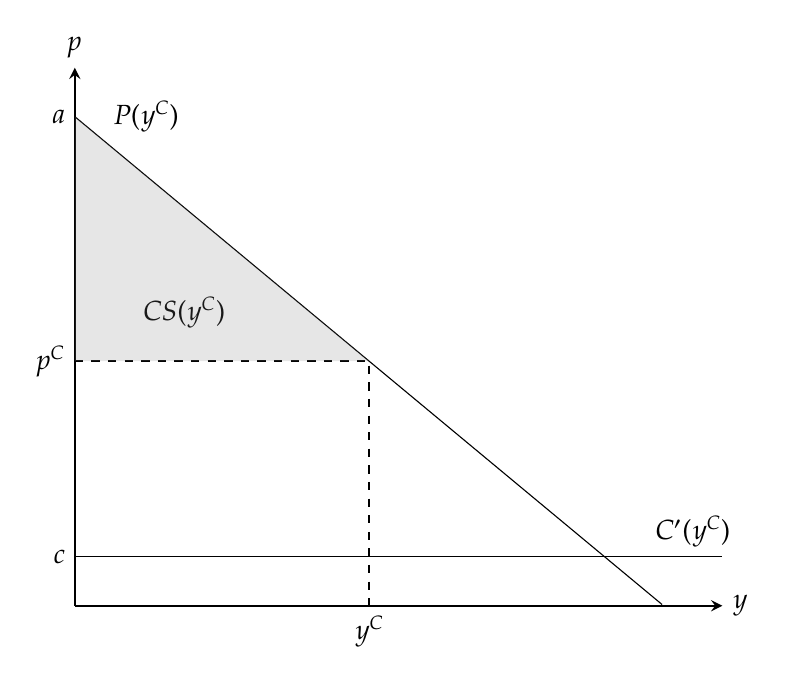
\begin{tikzpicture}
\figurename{}
\begin{axis}[
scale = 1.2,
xmin = 0, xmax = 11,
ymin = 0, ymax = 11,
axis lines = middle,
xtick = \empty , ytick = \empty,
clip = false,
axis line style = thick
]
\addplot[domain = 0:10, restrict y to domain = 0:10, samples = 400, color = black]{10-x};
\addplot[color = black, dashed, thick] coordinates {(0, 5) (5, 5) (5, 0)};
\addplot[color = black] coordinates {(0,1)(11,1)};
\node[right] at (current axis.right of origin){$y$};
\node [above] at (current axis.above origin){$p$};
\node [left] at (0, 5) {$p^C$};
\node [below] at (5, 0) {$y^C$};
\node [right] at (.5, 10) {$P(y^C)$};
\node [above] at (10.5, 1) {$C'(y^C)$};
\node [left] at (0, 10) {$a$};
\node [left] at (0,1) {$c$};
\node [right] at (1,6) {$CS(y^C)$};
\fill[gray, opacity = 0.2] (0, 10) -- (5, 5) -- (0,5);
\end{axis}
\end{tikzpicture}
\end{center}
\end{figure}
We focus now on solving the Stackelberg duopoly with the same parameters as in the Cournot duopoly, i.e. the inverse demand (\ref{eq:inv_suppl_sc}) and respectively costs and marginal costs (\ref{eq:costs_constant}) and (\ref{eq:mc_constant}). Inserting the various aforementioned functions into (\ref{eq:p_max_s}) given that  gives \begin{align}
\label{eq:stack_rapport}
0 &= a - by^S_1 - by^S_2 + y^S_1 \cdot (-b) - c \notag \\
y^S_1 & = \frac{a - c - by^S_2}{2b} \notag \\
& = \frac{a - c}{2b} - \frac{1}{2}y^S_2.
\end{align}

Using equality (\ref{eq:stack_rapport}) one can then solve the profit maximization equation (\ref{eq:max_duo_stack}) for firm 2, the follower, getting \begin{align}
0 &= a - b \cdot \left(\frac{a - c}{2b} - \frac{1}{2}y^S_2 \right) - by^S_2  + y^S_2 \cdot (-b) \cdot \left(\frac{(-b) - 0}{2 \cdot (-b) + 0 - 0}\right)\notag \\
by^S_2 & = \frac{1}{2} a - \frac{1}{2}c \notag \\
y^S_2 & = \frac{a - c}{2b}.
\end{align}
One can now solve equality (\ref{eq:stack_rapport}) by inserting the newly achieved $y^S_2$, obtaining \begin{align}
\label{eq:y_1_stack}
y^S_1 &= \frac{a - c}{2b} - \frac{1}{2} \cdot \left(\frac{a - c}{2b}\right)\notag \\
& = \frac{2a - 2c - a + c}{4b} \notag \\
& = \frac{a - c}{4b},
\end{align}
and as the total quantity $y^S = y^S_1 + y^S_2$ we get \begin{equation*}
y^S = \frac{3a - 3c}{4b}.
\end{equation*}
To get the price one only needs to insert $y^S$ into equation (\ref{eq:inv_suppl_sc}) that yields \begin{align}
p^S & = a - b \cdot \left(\frac{3a - 3c}{4b}\right)\notag \\
& = \frac{4a - 3a + 3c}{4} \notag \\
& = 	\frac{a + 3c}{4}.
\end{align}
Since now one has both the price and the individual quantities $y^S_1$ and $y^S_2$ one can start calculating the profit obtaining for firm 1: \begin{align*}
\pi(y^S_1) &= \left(\frac{a - c}{4b}\right) \cdot \left(\frac{a + 3c}{4}\right)\\
& = \frac{a^2 + 3ac - ac - 3c^2}{16b} + \frac{c^2 - ac}{4b}\\
& = \frac{a^2 + 2ac - 3c^2 + 4c^2 - 4ac}{16b}\\
& = \frac{a^2 - 2ac + c^2}{16b}\\
& = \frac{(a-c)^2}{16b}.
\end{align*}
Respectively for firm 2 the profit is \begin{align}
\label{eq:y^S_2}
\pi(y^S_2) &= \left(\frac{a - c }{2b}\right) \cdot \left(\frac{a + 3c}{4}\right) - c \cdot \left(\frac{a - c}{2b}\right) \notag \\
& = \frac{a^2 + 3ac - ac - 3c^2}{8b} + \frac{c^2 - ac}{2b}\notag \\
& = \frac{a^2 + 2ac - 3c^2 + 4c^2 - 4ac}{8b}\notag \\
& = \frac{a^2-2ac+c^2}{8b} \notag \\
& = \frac{(a-c)^2}{8b}.
\end{align}
Calculating now the total profit $\pi(y^S)$ yields \begin{align}
\label{eq:profit_stack}
\pi(y^S) &= \pi(y^S_1) + \pi(y^S_2) \notag \\
& = \frac{(a-c)^2}{16b} + \frac{2 \cdot (a-c)^2}{16b} \notag \\
& = \frac{3}{16b} \cdot (a - c)^2.
\end{align}

To compare both types of duopoly in a clarifying manner one needs to calculate again the consumer surplus with the price and quantities obtained with the aid of the Stackelberg's formulas. Using the same reasoning for the consumer surplus calculated in (\ref{eq:cons_surpl_cournot}) one gets: \begin{align}
\label{eq:cons_surpl_stack}
CS(y^S) & = \left(a - \left(\frac{a + 3c}{4}\right)\right) \cdot \left(\frac{3a - 3c}{4b}\right) \cdot \frac{1}{2} \notag \\
& = \left(\frac{(3a - 3c) \cdot (3a - 3c)}{16b}\right) \cdot \frac{1}{2} \notag \\
& = \frac{(3a - 3c)^2}{32b}.
\end{align}

One can already see substantial differences in the efficiency of the two duopolies in the case of constant marginal costs, and given that one judges the efficiency based on the firms point of view, it turns out that Cournot duopoly has a major advantage in respect of the total profits of the two firms and in minimizing consumer surplus. In fact using (\ref{eq:profit_courn}) and (\ref{eq:profit_stack}) one gets \begin{align*}
\pi(y^C) &> \pi(y^S)\\
\frac{2}{9b} \cdot (a - c)^2 &> \frac{3}{16b} \cdot (a - c)^2\\
\frac{2}{9b} &> \frac{3}{16b},
\end{align*}
instead using (\ref{eq:cons_surpl_cournot}) and (\ref{eq:cons_surpl_stack}) gives \begin{align*}
CS(y^C) &< CS(y^S)\\
\frac{(2a - 2c)^2}{18b} &< \frac{(3a - 3c)^2}{32b}\\
\frac{2}{9b} \cdot (a-c)^2 &<\frac{9}{32b} \cdot (a-c)^2\\
\frac{2}{9b} & < \frac{9}{32b}.
\end{align*}

One could also argue that $\pi(y^S_2) > \pi (y^C_i)$ for $i = 1,2$ based on (\ref{eq:y^S_2}) and (\ref{eq:profit_duo_s_c_1_2}), and thus that firm 2 as a follower would prefer a Stackelberg duopoly but if one reckons understands immediately that the advantage obtained is inferior compared to the edge that the Cournot duopoly has in the total profits. Hereafter we demonstrate it: \begin{align*}
\pi(y^S_2) &> \pi(y^C_i), \quad i = 1,2\\
\frac{(a - c)^2}{8b} &> \frac{(a -c)^2}{9b}\\
\frac{1}{8b} &> \frac{1}{9b},
\end{align*}
doing the percentage advantage gives \begin{align*}
\pi_{adv}(y^S_2) &= 1 - \left(\frac{1}{9b} \cdot \frac{8b}{1}\right)\\
& = \frac{1}{9} \approx 11.11 \%.
\end{align*}
but the disadvantage to be in the position of firm 1 as leader in a market with constant and identical marginal costs and linear inverse demand is: \begin{align*}
\pi(y^S_1) &< \pi(y^C_i), \quad i = 1,2\\
\frac{(a - c)^2}{16b} &< \frac{(a -c)^2}{9b}\\
\frac{1}{16b} &< \frac{1}{9b},
\end{align*}
thus yielding a percentage disadvantage of\begin{align*}
\pi_{dis}(y^S_1) &= \left(\frac{1}{16b} \cdot \frac{9b}{1}\right) - 1\\
& = -\frac{7}{16} = -43.75\%.
\end{align*}
Instead the edge that the Cournot duopoly model has on total profits is: \begin{align*}
\pi_{adv}(y^C) &= 1 - \left(\frac{3}{16b} \cdot \frac{9b}{2}\right)\\
& = \frac{5}{32} = 15.625\%,
\end{align*}

Given the results obtained, in such a market it would be in both firms interest to decide their quantities simultaneously and not sequentially, given the huge disadvantage that the firm that acts as a leader would have on their profits. 

The problem at economic level, however, also translates into a kind of ethical problem, in which competition within the free market is individualistic and unscrupulous, and thus the interest of the same companies is to maximize individually their profits, but also to remove any slice of market from the hands of the opponent. All this is even more evident in the situation of duopoly, in which because of these direct competition \emph{vis-à-vis}, the interdependence between the two companies causes great volatility of profits.
\newpage
\section{Conclusion}
This paper has certainly been a long journey, it has deepened Cournot's contributions to economic theory, it has shown that they were not only contributions that were later alienated and modified because reputed wrong, but fundamental pillars of modern economic theory, still valid today and even more surprisingly in the vanguard for the year, 1838, in which they were postulated and published. 

We were therefore able to outline in a clearer way, as has hardly been done so far to our knowledge, the respective links and congruencies between the concepts theorized by Cournot and modern microeconomic theory, which surprisingly were essentially identical at the empirical level and only different regarding the formulas, and of course of mathematical notation, but it is not difficult to imagine given the 184 years that separate us from the \emph{Recherches sur les principes mathématiques de la théorie des richesses}.

This paper has analyzed the situations in which the demand is linear and costs are identical, but further research could take as a starting point the results obtained from this paper and analyze more advanced microeconomic theories, to be able to define the influence of Cournot on them. In addition to this, the lack of empirical data on which to apply Cournot's theories is a strong deficiency in this paper, which is based primarily on algebraic calculus purely literal and therefore can not have a match in reality, thus a plausible empirical value. Having also dealt with Stackelberg has instead allowed to know more about the developments of Cournot duopoly theory has brought with it, and what advantages, which in the case were really inferior to disadvantages, belong to this type of duopoly compared to that of Cournot, although it would also be possible to compare it with the Bertrand duopoly.

On the whole, this work turns out to be only a starting point, and further study of the subject could lead to new interesting links between Cournot and current economic theory.

\newpage
\pagenumbering{Roman}
\setcounter{page}{3}

\bibliographystyle{apacite}
\bibliography{Bibliography}
\newpage
\thispagestyle{empty}
\section*{Declaration of Authorship}
I hereby declare\\
- that I have written this thesis without any help from others and without the use of documents 
or aids other than those stated above;\\
- that I have mentioned all the sources used and that I have cited them correctly according to 
established academic citation rules;\\
- that I have acquired any immaterial rights to materials I may have used, such as images or 
graphs, or that I have produced such materials myself;\\
- that the topic or parts of it are not already the object of any work or examination of another 
course unless this has been explicitly agreed to with the faculty member in advance and is 
referred to in the thesis;\\
- that I will not pass on copies of this work to third parties or publish them without the 
university’s written consent if a direct connection can be established with the University of 
St.Gallen or its faculty members;\\
- that I am aware that my work can be electronically checked for plagiarism and that I hereby 
grant the University of St.Gallen copyright in accordance with the Examination Regulations 
insofar as this is required for administrative action;\\
- that I am aware that the university will prosecute any infringement of this declaration of 
authorship and, in particular, the employment of a ghostwriter, and that any such infringement 
may result in disciplinary and criminal consequences which may result in my expulsion from the 
university or my being stripped of my degree.\\
\\
By uploading this academic term paper, I confirm through my conclusive action that I am submitting the Declaration of Authorship, that I have read and understood it, and that it is true.\\
\\
\\
Characters with spaces $\approx 41'979$\\
Elia A. G. Bucci
\end{document}
